\subsubsection{UC25 - Codice invita amici}
\begin{figure}[h]
	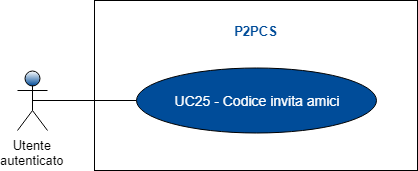
\includegraphics[width=9cm]{res/images/UC23Codiceamico.png}
	\centering
	\caption{UC25 - Codice invita amici}
\end{figure}
\begin{itemize}
	\item \textbf{Attori Primari}: utente autenticato;
	\item \textbf{Descrizione}: agli utenti autenticati è reso disponibile un codice personale alfanumerico che può essere inviato ad un amico, non ancora registrato, per invitarlo ad usufruire dell'applicazione semplicemente inserendo questo "codice amico" in fase di registrazione nell'apposito spazio facendo guadagnare così punti esperienza al proprietario del codice;
	\item \textbf{Scenario principale}: l'utente visualizza, nella voce \textit{Gestione Profilo} [UC14], il codice personale da inviare ad amici;
	\item \textbf{Precondizione}: l'utente autenticato ha selezionato la voce \textit{Gestione Profilo} [UC14] dal menu dell'applicazione;
	\item \textbf{Post-condizione}: l'utente autenticato ha visualizzato il suo codice personale. 
\end{itemize} 
